\documentclass[letterpaper, 10pt,titlepage]{article}

\usepackage[utf8]{inputenc}
\usepackage [english]{babel}
\usepackage [autostyle, english = american]{csquotes}
\usepackage{graphicx}                                        
\usepackage{amssymb}                                         
\usepackage{amsmath}                                         
\usepackage{amsthm}                                          
\usepackage{alltt}                                           
\usepackage{float}
\usepackage{url}
\newcommand\tab[1][1cm]{\hspace*{#1}}
\setlength{\parindent}{0em}
\setlength{\parskip}{1em}
\usepackage{pst-gantt}
\usepackage[letterpaper, margin=0.75in]{geometry}
\usepackage{balance}
\usepackage[TABBOTCAP, tight]{subfigure}
\usepackage{enumitem}
\usepackage{pstricks, pst-node}
\usepackage{hyperref}
\hypersetup{
  colorlinks = true,
  linkcolor  = black
}
\usepackage{listings}
\usepackage{color}
 
\definecolor{codegreen}{rgb}{0,0.6,0}
\definecolor{codegray}{rgb}{0.5,0.5,0.5}
\definecolor{codepurple}{rgb}{0.58,0,0.82}
\definecolor{backcolour}{rgb}{0.95,0.95,0.92}
 
\lstdefinestyle{mystyle}{
    backgroundcolor=\color{backcolour},   
    commentstyle=\color{codegreen},
    keywordstyle=\color{magenta},
    numberstyle=\tiny\color{codegray},
    stringstyle=\color{codepurple},
    basicstyle=\footnotesize,
    breakatwhitespace=false,         
    breaklines=true,                 
    captionpos=b,                    
    keepspaces=true,                 
    numbers=left,                    
    numbersep=5pt,                  
    showspaces=false,                
    showstringspaces=false,
    showtabs=false,                  
    tabsize=2
}
 
\lstset{style=mystyle}
\usepackage{minted}




\setcounter{secnumdepth}{4}
\def\name{Jiawei Liu}

\hypersetup{
  colorlinks = true,
  urlcolor = black,
  pdfauthor = {\name},
  pdfkeywords = {Problem Statement},
  pdftitle = {Capstone Project},
  pdfsubject = {Capstone Project},
  pdfpagemode = UseNone
}



\begin{document}

\begin{titlepage}
\begin{center}
    \Huge
    \textbf{The Preliminary Design Document}\\
    \textbf{Capstone Project}\\
    \vspace{1.0cm}
    \large
    Developers: Charles Henninger, Duncan Millard, Jiawei Liu\\
    Sponsor: Nancy Hildebrandt\\
    \vspace{1.5cm}
    \large
    Instructor: D. Kevin McGrath\\

    \large
    CS 461, Fall 2016, Oregon State University\\    

    \vspace{3.2cm}

    \large
    \underline{Abstract}\\
    \vspace{0.3cm}
    \end{center}
    \large

    \tab The Santiam wagon trail is historic trail located in the Willamette National Forest. The local ranger stations wish to have a mobile app that is capable of taking users on a tour of the wagon trail without needing a connection to the internet. The mobile application come in two forms: one developed for the Android mobile platform, and the other developed for the iOS mobile platform. While these two forms of the mobile application will be developed separately, they will be using the same methods of providing a tour to the user. The mobile application will render a map using a pre-downloaded map tile file and place waypoints onto the map that will be related to relevant information, in the form of videos and text files, about that area of the map. In order to achieve this functionality without internet access, we will rely on pre-downloaded content packs that will contain the map tiles, videos, text files, and waypoint information. These content packages will be created by staff of the local ranger stations, and uploaded via a website that will be developed along with the mobile app. Our team will divide these three larger sections of this project (the Android application, iOS application, and the Web Control panel/backend engineering) between the team members as follows: Android application development: Charles Henninger, Web Control panel/backend engineering: Duncan Millard, iOS application development: Jiawei Liu. This document outlines the possible technologies that will be used to address problems in each of these three major development sections, written by the team member heading each of the sections.
    
    \vspace{0.8cm}
    \vfill
    
\begin{center}    
    Dec 1, 2016

\end{center}
\end{titlepage}


\tableofcontents
\newpage



\section{Introduction}
\subsection{Purpose}
pending

\subsection{Scope}
pending
                                       
\subsection{Context}
pending

\subsection{Summary}
pending

\vspace{0.3cm}



\section{Glossary}
pending



\section{Body}
\subsection{Identified stakeholders and design concerns}
pending







\subsection{Design viewpoint: Context}
Do we need to introduce what is interface at here?

\subsubsection{Map rendering}
What must be accomplished in this part of the solution is making a map visible and capable of interaction with the user. We will need to display a relevant map of the tour area, capable of zooming, refocusing on the location of the user, and displaying waypoints on the map that contain relevant information about the area, including videos and text files. In order to get quality offline map tiles that we can use in our application, we have decided to use libraries connected to OpenStreetMaps, a project that provides free geographic data for use in rendering maps. OpenStreetMaps has many libraries that may provide us the means to render maps offline. At this point in time, we are planning on going with our second option, Mapbox GL, for implementation on both the IOS and Android platform. Mapbox GL is a free service that offers high quality rendering and mapping features offline, and brings with it many useful extra features such as custom waypoint and path editing. Charles Henninger will be leading the development of this piece of the solution


This aspect of our solution will almost entirely be under the viewpoint of information. After this piece is finished, Map Rendering will occur automatically once the User downloads a content package. As stated in another section of our design, the content package will contain a metadata file with information on the map needed for the tour. After receiving the completion signal for the download with the relevant download ID, our app will open the metadata file and pull a few pieces of information from it. We will get two sets of latitude and longitude points, the name of the area, and a list of waypoints, each containing their relevant information (meaning location on the map, identification number, and any video or text information). Using the two sets of latitude and longitude points, we will use the Mapbox library to create a download request for an offline map. The downloading itself will be handled by the Mapbox SDK. We will use the name of the area (found in the metadata file) to label the map. This offline map tile file will be organized and saved within the Mapbox directories, and will be edited via native services in the Mapbox Mapview class. We will create waypoints on our newly downloaded map via this Mapview class, using the waypoint data found in the metadata file. Once the map has been completed, our Mapview object can be placed in and statically manipulated by our UI.




\subsection{Design viewpoint: Interface}
Do we need to introduce what is interface at here?

\subsubsection{Android UI}
This piece of our solution will be the UI of the mobile app on the Android platform. We plan to conform to the Android UI guidelines for the layout of most of the UI. We have decided to use XML for our UI on our Android platform due to XML’s  simplicity, clarity, and speed compared to other options like Java or SDL. This section of our solution will be developed by Charles Henninger.


This portion of our application will be subject to the structure viewpoint. Once the app is opened, an XML file will display a menu of the tours currently downloaded will be shown to the User. The available tours will be listed as a list from top to bottom, one column and one tour in each row, ordered alphabetically by the name of the tour area. Swiping left on one of the tours will display an icon for deleting the tour, and an icon to display information on the tour. The information icon will bring up a small window detailing the size of the tour, and the number of waypoints located in the tour. The User can click an icon in the top left corner to display the menu for the app, or click on one of the available tours to display the map and waypoints for that tour. Both the menu button and available tour buttons will be Button XML objects that react with an onclick function. The menu will display buttons that, once clicked, will open the related XML file. Currently we plan on having menu buttons navigating to an available tours page (where the user can download new tours), a credits page (containing information on the developers), and a page displaying tours that have already been downloaded. The page for downloading new tours will be similar to the available tours page, with a list of tours organized by the name of the area they relate to. We will get this list via an API call to our server. Next to each tour will be a download icon that the User can click, if the tour has not already been downloaded, to begin the download for the tour files and the rendering of the map tiles for offline use. Navigating in to an available tour will open an XML file that will display the map of the area, complete with waypoints spread along the route. This map can be navigated by swiping across across the map to pan around the area, and pinching the map to zoom in/out. Clicking on the map will cause the application to check the coordinates of the area clicked. If the area matches a waypoint latitude and longitude values, then a menu will be displayed below the map containing that waypoints information, including videos and text files. Clicking back on the map will close this menu. All of what is described here is completed in XML with buttons and onclick events, with some calls to other sections of the app to get relevant information (such as using the Mapbox element’s native functions to cause the map to pan and zoom). Lastly, our credits page will be a simple XML file with text introducing the developers and perhaps a short message to the user.



\subsubsection{iOS UI}
One of the platforms that we will be designing on for this project is the iOS platform. Due to the nature of this project, the usability of the mobile app is an important part of the project. In this iOS user interface design section, we will discuss the different options for handling problems such as designing and implementing the UI for selecting content packages, downloading and removing them, as well as basics for tour layout. For solving these problems, I choose Xcode as the solution.

Xcode is an integrated development environment (IDE) that developed by Apple. Developers can use Xcode to develop both iOS and macOS applications. The purpose of using Xcode is to design and implement the UI by a tool or a IDE, Due to the high integration of Xcode, this can bring some convenient and save our time to build the development environment.

In order to use Xcode for Swift, it is necessary in order to get acquainted with Xcode. As Figure 1 show, Xcode has the object library on the right side, and allow developers to drag an object from the library to the application. There are not that many techniques in the UI design section, it basically selects the object from the library and drags it to the design area. It is simple and visible. Xcode is the official IDE for developing iOS application, and is offered for free. Therefore, most iOS applications are developed by Xcode. For example, Safari, eBay, Expedia, etc.

\begin{figure}[ht]
    \centering
    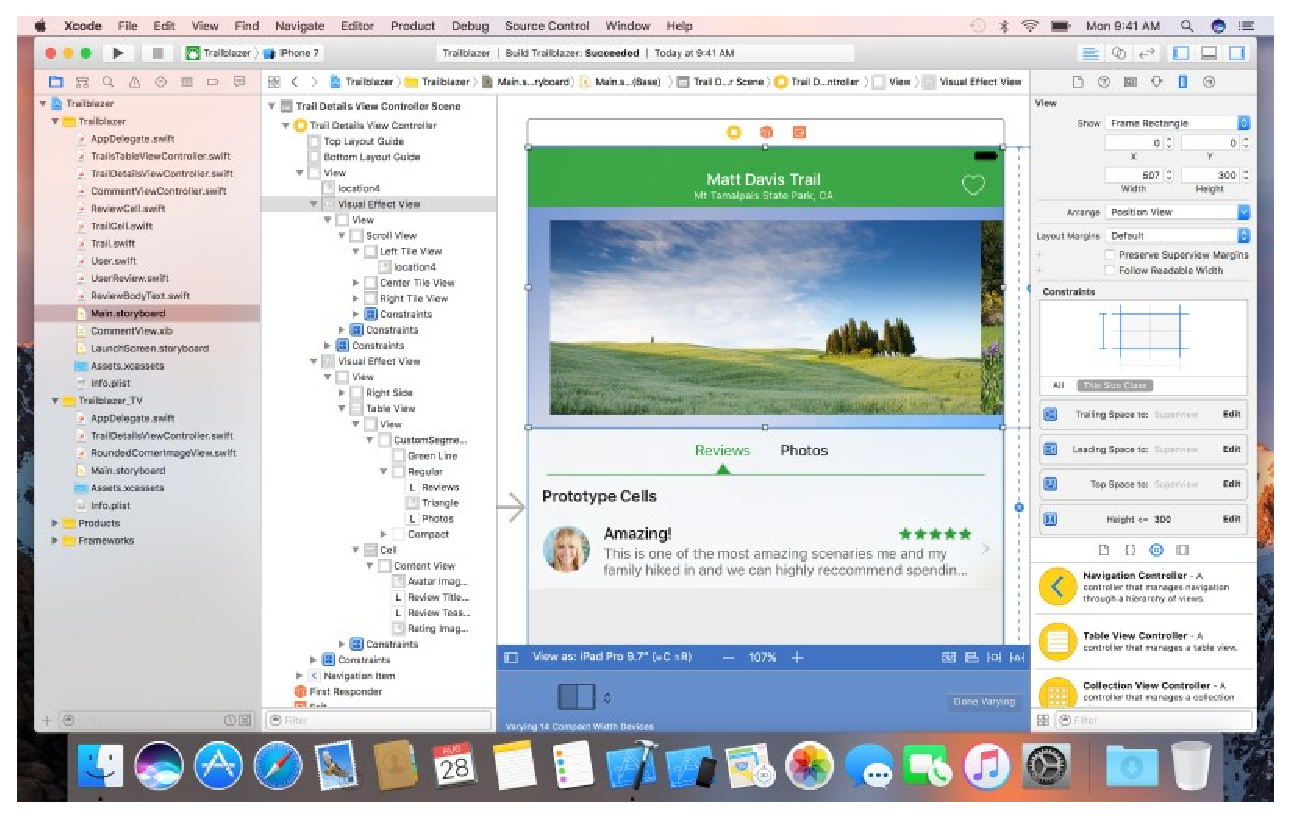
\includegraphics[scale=0.5]{j1}
    \caption{Xcode Interface [1]}
    \label{jiawei1}
\end{figure}

When I start to design iOS application UI, I will create a new project in Xcode first. Xcode includes many built-app templates for developing iOS apps, such as tabbed application, game and page-based application. For this project, I will use single view application to start our project. Then, Xcode will show a dialog to let me name the app and choose additional options. After these setting steps, the Xcode will show the design interface which similarity with Figure 1. For our project, I will drag the necessary objects from the library to the application. I will add a few (3 or 4) buttons on the bottom of application to separate functions into different sections. In addition, since we are designing a map application, I will show the map on the home page with user’s location and viewpoints. Here is a rough iOS UI for our project.

\begin{figure}[ht]
    \centering
    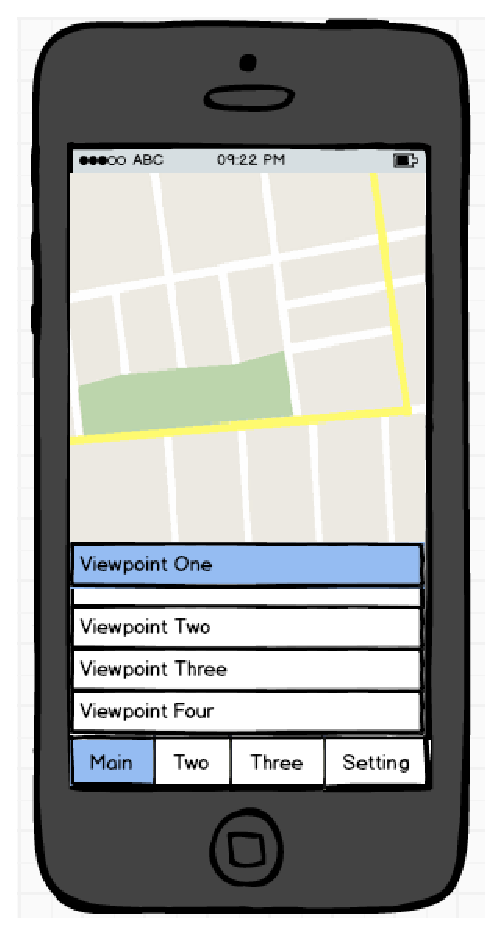
\includegraphics[scale=0.5]{j2}
    \caption{Rough iOS UI}
    \label{jiawei2}
\end{figure}

For design the UI, I will drag a Map View from Object Library to the view controller and use MapKit API display the map with user’s location on the home screen, and list the viewpoints under the map. On the bottom of app, there are four (or less) menus to classify all function. For example, since our project need to download content packages for using app without network connection, the downloading/removing content package function will in the setting menu. In a word, I will create iOS app UI by dragging the relevant object from the library to the application to make the UI easy to use and understand.


\subsubsection{Web Control Panel UI}
What has to be accomplished in this part of the solution is designing and implementing the tour creation. We need to design a website to allow administrators such as our client, Nancy to setup for map frame, click to add waypoints, click waypoints to add texts and videos. In order to control resource on the web, we need to design a dynamic website with a clear UI. Therefore, we are going to use Bootstrap and jQuery to create web control panel UI. 


Bootstrap is the most popular HTML, CSS, and JavaScript framework for developing responsive, mobile-first web sites [2]. In addition, Bootstrap is offered for free. Everybody can download and use it. The purpose of using Bootstrap is creating a dynamic website as the web control panel for our client to control online texts and videos resources. 


In general, syntax of Bootstrap is similar with HTML technique. However, Bootstrap is more powerful than HTML because it provided more functions such as preprocessors and universal framework. In addition, as Figure 3 show, there are abundant themes available for free. We can apply these themes to create the website with an aesthetically pleasing UI. As the most popular framework for developing websites, there are a number of websites are using Bootstrap, such as NBA.com, Walmart, gliffy, etc.

\begin{figure}[ht]
    \centering
    \includegraphics[scale=0.4]{j3}
    \caption{Free Bootstrap Templates [3]}
    \label{jiawei3}
\end{figure}

jQuery is a library of JavaScript. The purpose of using jQuery is it easy to learn and apply in the web page. The jQuery library contains these features, which are HTML/DOM manipulation, CSS manipulation, HTML event methods, Effects and animations, AJAX and Utilities [4]. With jQuery, developers can write less code to achieve the same goal on web pages. 


Since jQuery is a JavaScript library and has many features of HTML, it based on JavaScript, HTML and CSS. We can consider jQuery as a highly-integrated development tool to simplify web development process. jQuery is a necessary technology for developing dynamic web pages. Therefore, a lot of famous websites used jQuery, such as Google Maps, Google Doc, Netflix, etc.

\begin{figure}[ht]
    \centering
    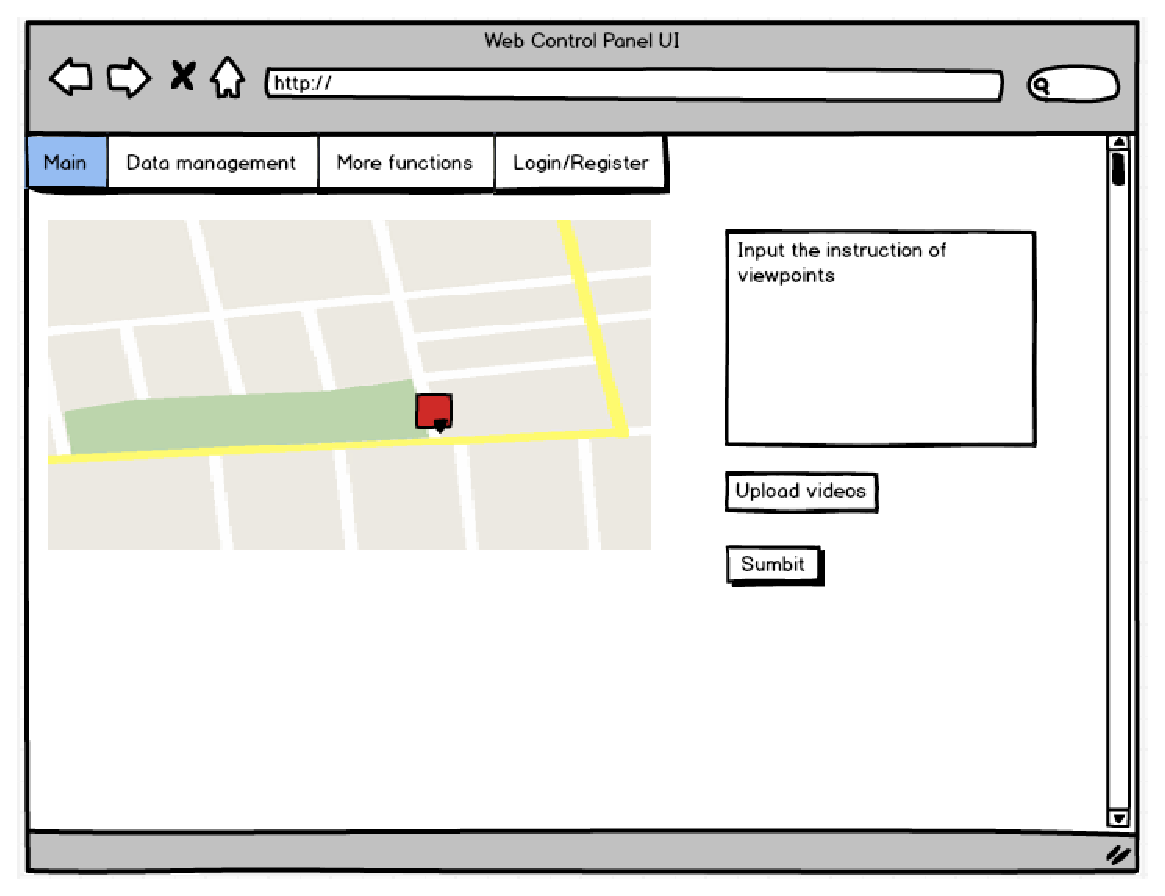
\includegraphics[scale=0.5]{j4}
    \caption{Rough Web Control Panel UI}
    \label{jiawei4}
\end{figure}

For design the Web Control Panel UI, I will start with a bare Bootstrap template, which only contains a navigation bar at the top. I provide a rough web control panel UI (Figure 4), the basic operation logic will be similarly with my iOS UI, which is display the map on the main page. After login/register, the administrator will be able to add new viewpoints with text instructions and videos. Once the administrator input all information of the viewpoints, the administrator just click “Submit” button to upload all information into our database. For displaying the map, I will use Bootstrap to leave an area and use jQuery to make the map dynamic and operable. On the navigation bar, I will add a few HTML buttons for providing more functions. For example, a webpage to let administrator modify the viewpoint which already saved in the database. I will use a HTML form to display all saved viewpoints and let the administrator to edit them. In a word, Bootstrap is the main method to design the layout of web control panel UI, and jQuery is the main method to make the map dynamic and operable.


\subsection{Design viewpoint: Interaction}

\subsubsection{Android Remote API Interactions}
This piece of our solution involves how we will download our content package files from our server onto the mobile device. Users will view available content packs in app and select which content packs that they want to download. Once a user confirms a download, the mobile app will make an API call to our web server and begin downloading the file. the service that we use for downloading files on the Android platform will be DownloadManager, which is a native Android service that is meant for larger files that require long running downloads and comes with many build in features, such as notifications for completed downloads, that would have to be manually added with other services. This section of our solution will be developed by Charles Henninger.


Our Remote API interactions will on the Android platform (meaning requesting a download for the tour files from our server) will be under an interaction perspective and occur when the User confirms the download of a currently undownloaded tour. Once this happens, we will use the native DownloadManager class to make an HTTP download request to our server. From here, all we have to do is let DownloadManager handle the file download, and indicate an action when the file is completed. This action will initiate the map rendering process to begin, which will use Mapbox and a metadata file located in the newly downloaded tour file to create an offline map.



\subsubsection{iOS Remote API Interactions}
In this section, we are going to provide a solution that allows users download content packages to their iOS devices. Users also permit to see all available content packages and select the package that they wish to download. After users choose the package, the application start to download the package by making an API call to the web server. To achieve this goal, we have two technologies available, which are WKWebView and NSURLConnection.


WKWebView is a class of iOS to interactive web content, such as for an in-app browser [5]. The purpose of using WKWebView object in our application is interactive with our server and load content package list for users. There is a symbol in WKWebView called loading content. With this symbol, we are able to set the webpage contents and base URL for users, then the user can select and download the package. Here is an example about creating a WKWebView programmatically [5].

\begin{minted}{swift}
import UIKit
import WebKit
class ViewController: UIViewController, WKUIDelegate {
    
    var webView: WKWebView!
    
    override func loadView() {
        let webConfiguration = WKWebViewConfiguration()
        webView = WKWebView(frame: .zero, configuration: webConfiguration)
        webView.uiDelegate = self
        view = webView
    }
    override func viewDidLoad() {
        super.viewDidLoad()
        
        let myURL = URL(string: "https://www.apple.com")
        let myRequest = URLRequest(url: myURL!)
        webView.load(myRequest)
    }}
\end{minted}


WKWebView was starting at iOS 8. It is based on iOS operating system. Besides, most iOS web browsers and in-app browsers are using WKWebView. For example, Safari and Twitter’s in-app browser. WKWebView is popular and necessary for iOS development.


NSURLConnection is similar with WKWebView. It is also a class iOS. A NSURLConnection object lets you load the contents of a URL by providing a URL request object [6]. Therefore, the purpose of using NSURLConnection is loading content packages from the web server by a URL request. 


As a class of iOS, it is built on iOS operating system, and has its own syntax. Most iOS applications are using NSURLConnection to connect to server and load packages. For example, some huge iOS games are required download data packages to the device. These games used NSURLConnection technology. And then, this situation is analogous with downloading content packages to iOS devices.


In our application, we are going to use WKWebView class to display the available package data from our server. First, I will create a new WKWebView object using the init(frame:configuration:) method. And then, I will use the load(\_:) method to begin loading web content from our server and display all available content packages. If the user wants to stop loading the page, I will provide a stop button by stopLoading() method to stop loading. As Listing 1 show, I will include my URL in the code and begin to load the content by an API call. In addition, we are going to utilize NSURLConnection technics to download content packages from the web server. I will create a URL connection object with a delegate object that conforms to the NSURLConnectionDelegate and NSURLConnectionDataDelegate protocols. And then, once the user selects the content package, the app will send a request to the server. In detail, the NSURLConnectionDelegate protocol is mainly used for credential handling, but also handles connection completion. connection(\_:willSendRequestFor:) is the actual method to send requires. We just replace with our URL in the code, the request will send to our server and start to download the content package.



\subsection{Design viewpoint: ???}

\subsubsection{???}
context is here















\section{Design rationale}
pending



\section{Conclusion}
The unifying feature of each of our individual design pieces was the need for clarity and ease of use. This app will be used and maintained predominantly by people that have little to no developmental experience. Because of this, we must focus our designs to be simple to understand and use. 









































\newpage %add references at here
\begin{thebibliography}{9}

%%
\bibitem{1} 
"Apple," \textit{Interface Builder Built-In}. [Online]. Available:
\texttt{https://developer.apple.com/xcode/interface-builder/} [Accessed: 14-Nov-2016].
%%
\bibitem{2} 
"w3schools," \textit{Bootstrap 3 Tutorial}. [Online]. Available:
\texttt{http://www.w3schools.com/bootstrap/} [Accessed: 14-Nov-2016].
%%
\bibitem{3} 
"Start Bootstrap," \textit{All Templates}. [Online]. Available:
\texttt{https://startbootstrap.com/template-categories/all/} [Accessed: 14-Nov-2016].
%%
\bibitem{4} 
"w3schools," \textit{jQuery Introduction}. [Online]. Available:
\texttt{http://www.w3schools.com/jquery/jquery\_intro.asp} [Accessed: 14-Nov-2016].
%%
\bibitem{5} 
"Apple Developer," \textit{WKWebView}. [Online]. Available:
\texttt{https://developer.apple.com/reference/webkit/wkwebview} [Accessed: 14-Nov-2016].
%%
\bibitem{6} 
"Apple Developer," \textit{NSURLConnection}. [Online]. 
\\Available: \texttt{https://developer.apple.com/reference/foundation/nsurlconnection} [Accessed: 14-Nov-2016].
%%














\end{thebibliography}
\end{document}
